\section{排序关系}
不同于等价关系,\DefineConcept{排序关系}(ordering relation)具有一些别致的性质.

\subsection{偏序关系}
\begin{definition}
%@see: 《Elements of Set Theory》 P168 Definition
设\(\rel{R}\)是集合\(A\)上的一个二元关系.
如果\(\rel{R}\)具有\emph{自反性}、\emph{反对称性}和\emph{传递性},
那么称“\(\rel{R}\)是\(A\)上的\DefineConcept{偏序关系}(partial ordering)”,
称“\(A\)是\DefineConcept{偏序集}(partially ordered set)”.
% partially ordered set 简称 poset
%@see: https://mathworld.wolfram.com/PartiallyOrderedSet.html
%@see: https://math.berkeley.edu/~wodzicki/H104.F10/OrderedSets.pdf
\end{definition}

\begin{definition}
设\(\rel{R}\)是集合\(A\)上的一个二元关系.
如果\(\rel{R}\)具有\emph{传递性},但不具有\emph{自反性},
那么称“\(\rel{R}\)是\(A\)上的\DefineConcept{严格偏序关系}(strict partial ordering)”,
称“\(A\)是\DefineConcept{严格偏序集}(strictly partially ordered set)”.
\end{definition}

\begin{definition}
设\(\opair{A,\leq}\)是一个偏序集.
若\(x \nleq y\)且\(y \nleq x\),
则称“\(x\)与\(y\)~\DefineConcept{不可比较}(\(x\) and \(y\) are \emph{incomparable})”;
否则称“\(x\)与\(y\)~\DefineConcept{可以比较}(\(x\) and \(y\) are \emph{comparable})”.
%@see: http://www.math.clemson.edu/~macaule/classes/m22_math4190/slides/math4190_lecture-04-03_h.pdf
\end{definition}

\begin{example}
%@see: 《Real Analysis Modern Techniques and Their Applications Second Edition》 P5
设\(A\)是集合,
则\(\subseteq\)是\(\Powerset A\)上的偏序关系.
\end{example}

\subsection{哈斯图}
%@see: 《离散数学及其应用(原书第7版)》 P521
我们可以用有向图描绘有限偏序集,
只需要将每个元素按照偏序关系规定的顺序依次排开,
再用有向弧连接每一对元素.
例如,在集合\(\{1,2,3,4\}\)上定义偏序关系\[
	\Set{\opair{a,b} \given a \leq b}
	= \Set{
		\opair{1,1},
		\opair{2,2},
		\opair{3,3},
		\opair{4,4},
		\opair{1,2},
		\opair{2,3},
		\opair{3,4},
		\opair{1,3},
		\opair{2,4},
		\opair{1,4}
	},
\]
那么可以得到如\cref{figure:偏序关系.有向图1} 所示的有向图.
应该注意到,在这个有向图中,在每一个顶点处都有环,
鉴于它们必定出现,所以我们不必画出这些环.
由于偏序关系具有传递性,所以我们不必画出那些可以利用传递性得到的弧
(例如\(\opair{1,3},
\opair{2,4},
\opair{1,4}\)这三段弧).
如果我们假设所有弧的方向都是大体向上,那么我们也不必标注弧的方向.
通过上述三种手段,我们就能让画面更加简洁,得到\cref{figure:偏序关系.哈斯图1}.

\begin{figure}[hbt]
	\centering
	\tikzset{
		%@see: https://tex.stackexchange.com/a/69225
		on each segment/.style={
			decorate,
			decoration={
				show path construction,
				moveto code={},
				lineto code={
					\path [#1]
					(\tikzinputsegmentfirst) -- (\tikzinputsegmentlast);
				},
				curveto code={
					\path [#1] (\tikzinputsegmentfirst)
					.. controls
					(\tikzinputsegmentsupporta) and (\tikzinputsegmentsupportb)
					..
					(\tikzinputsegmentlast);
				},
				closepath code={
					\path [#1]
					(\tikzinputsegmentfirst) -- (\tikzinputsegmentlast);
				},
			},
		},
		% style to add an arrow in the middle of a path
		mid arrow/.style={postaction={decorate,decoration={
			markings,
			mark=at position .5 with {\arrow[#1]{stealth}}
		}}},
	}
	\def\subwidth{.4\linewidth}
	\begin{subfigure}[b]{\subwidth}
		\centering
		\begin{tikzpicture}
			\tikzstyle{midarrow}=[draw=blue,postaction={on each segment={mid arrow=red}}]
			\draw[midarrow] (0,1)to(0,2);
			\draw[midarrow] (0,2)to(0,3);
			\draw[midarrow] (0,3)to(0,4);
			\draw[midarrow] (0,1)to[out=135,in=225](0,4);
			\draw[midarrow] (0,1)to[out=113,in=247](0,3);
			\draw[midarrow] (0,2)to[out=113,in=247](0,4);
			\draw[midarrow] (0,1)++(.25,0)circle(.25);
			\draw[midarrow] (0,2)++(.25,0)circle(.25);
			\draw[midarrow] (0,3)++(.25,0)circle(.25);
			\draw[midarrow] (0,4)++(.25,0)circle(.25);
			\fill(0,1)circle(2pt)node[right]{1};
			\fill(0,2)circle(2pt)node[right]{2};
			\fill(0,3)circle(2pt)node[right]{3};
			\fill(0,4)circle(2pt)node[right]{4};
		\end{tikzpicture}
		\caption{}
		\label{figure:偏序关系.有向图1}
	\end{subfigure}~\begin{subfigure}[b]{\subwidth}
		\centering
		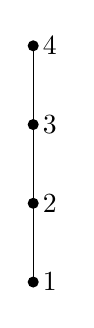
\begin{tikzpicture}
			\fill(0,1)circle(2pt)node[right]{1};
			\fill(0,2)circle(2pt)node[right]{2};
			\fill(0,3)circle(2pt)node[right]{3};
			\fill(0,4)circle(2pt)node[right]{4};
			\draw(0,1)--(0,4);
		\end{tikzpicture}
		\caption{}
		\label{figure:偏序关系.哈斯图1}
	\end{subfigure}
\end{figure}

总结一下,我们可以使用下面的过程
表示一个有限的偏序集\(\opair{S,\leq}\):\begin{enumerate}
	\item 从偏序关系中去掉所有的环
	(即\(\Set{\opair{a,a} \given a \in S}\));
	\item 去掉所有可以利用传递性得到的弧
	(即\(\Set{\opair{a,c} \given (\exists b \in S)[a < b \land b < c]}\);
	\item 排列每条弧,使得它的起点在终点下面,擦除弧上的箭头.
\end{enumerate}
我们把按照上述步骤绘制得到的图称为“偏序集\(\opair{S,\leq}\)的\DefineConcept{哈斯图}”.
它是以德国数学家赫尔姆·哈斯的名字命名的.

\begin{definition}
%@see: 《离散数学及其应用(原书第7版)》 P521
设\(\opair{A,\leq}\)是偏序集,\(x,y \in A\).
若\(x < y\),且不存在\(z \in S\)使得\(x < z < y\),
则称“\(y\)覆盖\(x\)”.
把\[
	\Set{\opair{x,y} \in A^2 \given \text{$y$覆盖$x$}}
\]称为“\(\opair{A,\leq}\)的\DefineConcept{覆盖关系}”.
\end{definition}

\subsection{最大元,最小元,上界,下界}
\begin{definition}
%@see: 《Real Analysis Modern Techniques and Their Applications Second Edition》 P5
设\(X\)是非空集合,
\(x \in X\),
\(E \subseteq X\),
\(\rel{R}\)是\(X\)上的偏序关系.

我们如果把满足\[
	[y \in X \implies x\rel{R}y]
	\implies
	y = x,
\]的\(x\)称为
“\(X\)(关于\(\mathcal{R}\))的\DefineConcept{最大元}”
或“\(\opair{X,\mathcal{R}}\)的\DefineConcept{最大元}(maximal element)”,
那么相应地把满足\[
	[y \in X \implies y\rel{R}x]
	\implies
	y = x,
\]的\(x\)称为
“\(X\)(关于\(\mathcal{R}\))的\DefineConcept{最小元}”
或“\(\opair{X,\mathcal{R}}\)的\DefineConcept{最小元}(minimal element)”.

在上述约定下,
如果\(x\)满足\[
	(\forall y \in E)[y\rel{R}x],
\]
那么称“\(x\)是\(E\)(在\(\opair{X,\mathcal{R}}\)中)的\DefineConcept{上界}(upper bound)”.
如果\(x\)满足\[
	(\forall y \in E)[x\rel{R}y],
\]
那么称“\(x\)是\(E\)(在\(\opair{X,\mathcal{R}}\)中)的\DefineConcept{下界}(lower bound)”.
\end{definition}

\begin{example}
我们知道\(\leq\)是区间\(X=[0,1]\)上的偏序关系.
易见\(1\)既是\(X\)(关于\(\leq\))的最大元,又是\([0,1]\)的上界;
而\(0\)既是\(X\)(关于\(\leq\))的最小元,又是\([0,1]\)的下界.
\end{example}

\subsection{线性序}
\begin{definition}
%@see: 《Elements of Set Theory》 P62 Definition
设\(\rel{R}\)是集合\(A\)上的一个二元关系.
如果\begin{enumerate}
	\item \(\rel{R}\)具有传递性,
	\item \(\rel{R}\)在\(A\)上服从\DefineConcept{三一律}(trichotomy),
	也就是说,对于\(\forall x,y \in A\),
	在以下三个命题中,有且仅有一个是真命题:\[
		x \rel{R} y, \qquad
		x = y, \qquad
		y \rel{R} x;
	\]
	%@see: https://mathworld.wolfram.com/TrichotomyLaw.html
\end{enumerate}
那么称\(\rel{R}\)为
“\(A\)上的\DefineConcept{线性序}(linear ordering)
或\DefineConcept{全序}(total ordering)”.
\end{definition}

应该注意到,当\(x = y\)时,三一律要求\[
	x \rel{R} x, \qquad
	x = x, \qquad
	x \rel{R} x
\]中的一个成立,
考虑到\(x = x\)恒成立,
那么必有\(x \rel{R} x\)恒不成立.
易见当\(x \neq y\)时,必有\(x \rel{R} y\)或\(y \rel{R} x\)之一成立,
都不可能有\(x \rel{R} y\)和\(y \rel{R} x\)都成立.
于是我们证得如下定理.

\begin{theorem}
%@see: 《Elements of Set Theory》 P63 Theorem 3R
设\(\rel{R}\)是集合\(A\)上的线性序.
\begin{enumerate}
	\item \(\rel{R}\)不具有自反性,
	即不存在\(x\)使得\(x \rel{R} x\).

	\item \(\rel{R}\)在\(A\)上是连通的(\(\rel{R}\) is \emph{connected} on \(A\)),
	即对于不同的\(x,y \in A\),要么有\(x \rel{R} y\)成立,要么有\(y \rel{R} x\)成立.
\end{enumerate}
\end{theorem}

值得注意的是,
线性序\(\rel{R}\)永远不会给出如下的环形:
\begin{center}
	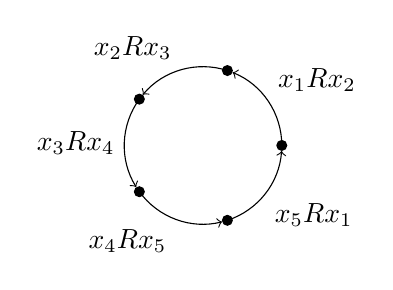
\begin{tikzpicture}
		\fill(1,0)circle(2pt)coordinate(A0);
		\fill({cos(72)},{sin(72)})circle(2pt)coordinate(A1);
		\fill({cos(144)},{sin(144)})circle(2pt)coordinate(A2);
		\fill({cos(216)},{sin(216)})circle(2pt)coordinate(A3);
		\fill({cos(288)},{sin(288)})circle(2pt)coordinate(A4);
		\begin{scope}[->]
			\draw(A0)arc[start angle=0,end angle=68,radius=1]node[midway,above right]{\(x_1 \rel{R} x_2\)};
			\draw(A1)arc[start angle=72,end angle=140,radius=1]node[midway,above left]{\(x_2 \rel{R} x_3\)};
			\draw(A2)arc[start angle=144,end angle=212,radius=1]node[midway,left]{\(x_3 \rel{R} x_4\)};
			\draw(A3)arc[start angle=216,end angle=284,radius=1]node[midway,below left]{\(x_4 \rel{R} x_5\)};
			\draw(A4)arc[start angle=288,end angle=356,radius=1]node[midway,below right]{\(x_5 \rel{R} x_1\)};
		\end{scope}
	\end{tikzpicture}
\end{center}
这是因为,如果我们有这样的环形成立,
那么根据传递性必有\(x_1 \rel{R} x_1\),
而这就与反自反性矛盾!

\begin{example}
设\(\rel{R}\)是\(A\)上的一个线性序,
证明:\(\rel{R}^{-1}\)也是\(A\)上的线性序.
\begin{proof}
由于\[
	\bigl( x \rel{R} y \land y \rel{R} z \implies x \rel{R} z \bigr)
	\iff
	\bigl( y \rel{R}^{-1} x \land z \rel{R}^{-1} y \implies z \rel{R}^{-1} x \bigr),
\]
可知\(\rel{R}^{-1}\)具有传递性.
又因为\(\rel{R}\)是\(A\)上的线性序,
所以对于\(\forall x,y \in A\),以下三个命题\[
	x \rel{R} y, \qquad
	x = y, \qquad
	y \rel{R} x
\]有且仅有一个成立;
换句话说,以下三个命题\[
	y \rel{R}^{-1} x, \qquad
	x = y, \qquad
	x \rel{R}^{-1} y
\]有且仅有一个成立;
可知\(\rel{R}^{-1}\)服从三一律.
综上所述,\(\rel{R}^{-1}\)也是\(A\)上的线性序.
\end{proof}
\end{example}
